% Options for packages loaded elsewhere
\PassOptionsToPackage{unicode}{hyperref}
\PassOptionsToPackage{hyphens}{url}
%
\documentclass[
  english,
  man,floatsintext]{apa6}
\usepackage{lmodern}
\usepackage{amssymb,amsmath}
\usepackage{ifxetex,ifluatex}
\ifnum 0\ifxetex 1\fi\ifluatex 1\fi=0 % if pdftex
  \usepackage[T1]{fontenc}
  \usepackage[utf8]{inputenc}
  \usepackage{textcomp} % provide euro and other symbols
\else % if luatex or xetex
  \usepackage{unicode-math}
  \defaultfontfeatures{Scale=MatchLowercase}
  \defaultfontfeatures[\rmfamily]{Ligatures=TeX,Scale=1}
\fi
% Use upquote if available, for straight quotes in verbatim environments
\IfFileExists{upquote.sty}{\usepackage{upquote}}{}
\IfFileExists{microtype.sty}{% use microtype if available
  \usepackage[]{microtype}
  \UseMicrotypeSet[protrusion]{basicmath} % disable protrusion for tt fonts
}{}
\makeatletter
\@ifundefined{KOMAClassName}{% if non-KOMA class
  \IfFileExists{parskip.sty}{%
    \usepackage{parskip}
  }{% else
    \setlength{\parindent}{0pt}
    \setlength{\parskip}{6pt plus 2pt minus 1pt}}
}{% if KOMA class
  \KOMAoptions{parskip=half}}
\makeatother
\usepackage{xcolor}
\IfFileExists{xurl.sty}{\usepackage{xurl}}{} % add URL line breaks if available
\IfFileExists{bookmark.sty}{\usepackage{bookmark}}{\usepackage{hyperref}}
\hypersetup{
  pdftitle={Supplimental analyses for: Emotional information-processing correlates of positive mental health in adolescence: A network analysis approach},
  hidelinks,
  pdfcreator={LaTeX via pandoc}}
\urlstyle{same} % disable monospaced font for URLs
\usepackage{graphicx,grffile}
\makeatletter
\def\maxwidth{\ifdim\Gin@nat@width>\linewidth\linewidth\else\Gin@nat@width\fi}
\def\maxheight{\ifdim\Gin@nat@height>\textheight\textheight\else\Gin@nat@height\fi}
\makeatother
% Scale images if necessary, so that they will not overflow the page
% margins by default, and it is still possible to overwrite the defaults
% using explicit options in \includegraphics[width, height, ...]{}
\setkeys{Gin}{width=\maxwidth,height=\maxheight,keepaspectratio}
% Set default figure placement to htbp
\makeatletter
\def\fps@figure{htbp}
\makeatother
\setlength{\emergencystretch}{3em} % prevent overfull lines
\providecommand{\tightlist}{%
  \setlength{\itemsep}{0pt}\setlength{\parskip}{0pt}}
\setcounter{secnumdepth}{-\maxdimen} % remove section numbering
% Make \paragraph and \subparagraph free-standing
\ifx\paragraph\undefined\else
  \let\oldparagraph\paragraph
  \renewcommand{\paragraph}[1]{\oldparagraph{#1}\mbox{}}
\fi
\ifx\subparagraph\undefined\else
  \let\oldsubparagraph\subparagraph
  \renewcommand{\subparagraph}[1]{\oldsubparagraph{#1}\mbox{}}
\fi
% Manuscript styling
\usepackage{upgreek}
\captionsetup{font=singlespacing,justification=justified}

% Table formatting
\usepackage{longtable}
\usepackage{lscape}
% \usepackage[counterclockwise]{rotating}   % Landscape page setup for large tables
\usepackage{multirow}		% Table styling
\usepackage{tabularx}		% Control Column width
\usepackage[flushleft]{threeparttable}	% Allows for three part tables with a specified notes section
\usepackage{threeparttablex}            % Lets threeparttable work with longtable

% Create new environments so endfloat can handle them
% \newenvironment{ltable}
%   {\begin{landscape}\begin{center}\begin{threeparttable}}
%   {\end{threeparttable}\end{center}\end{landscape}}
\newenvironment{lltable}{\begin{landscape}\begin{center}\begin{ThreePartTable}}{\end{ThreePartTable}\end{center}\end{landscape}}

% Enables adjusting longtable caption width to table width
% Solution found at http://golatex.de/longtable-mit-caption-so-breit-wie-die-tabelle-t15767.html
\makeatletter
\newcommand\LastLTentrywidth{1em}
\newlength\longtablewidth
\setlength{\longtablewidth}{1in}
\newcommand{\getlongtablewidth}{\begingroup \ifcsname LT@\roman{LT@tables}\endcsname \global\longtablewidth=0pt \renewcommand{\LT@entry}[2]{\global\advance\longtablewidth by ##2\relax\gdef\LastLTentrywidth{##2}}\@nameuse{LT@\roman{LT@tables}} \fi \endgroup}

% \setlength{\parindent}{0.5in}
% \setlength{\parskip}{0pt plus 0pt minus 0pt}

% \usepackage{etoolbox}
\makeatletter
\patchcmd{\HyOrg@maketitle}
  {\section{\normalfont\normalsize\abstractname}}
  {\section*{\normalfont\normalsize\abstractname}}
  {}{\typeout{Failed to patch abstract.}}
\makeatother
\shorttitle{supplimental analyses}
\author{Sam Parsons\textsuperscript{1}, Annabel Songco\textsuperscript{1}, Charlotte Booth\textsuperscript{1}, \& Elaine Fox\textsuperscript{1}}
\affiliation{
\vspace{0.5cm}
\textsuperscript{1} Department of Experimental Psychology, University of Oxford}
\authornote{author note


Correspondence concerning this article should be addressed to Sam Parsons, Department of Experimental Psychology, University of Oxford, New Radcliffe House, Radcliffe Observatory Quarter, Oxford, OX2 6AE. E-mail: sam.parsons@psy.ox.ac.uk}
\usepackage{lineno}

\linenumbers
\usepackage{csquotes}
\usepackage{float}
\floatplacement{figure}{H}
\raggedbottom
\note{\clearpage}
\ifxetex
  % Load polyglossia as late as possible: uses bidi with RTL langages (e.g. Hebrew, Arabic)
  \usepackage{polyglossia}
  \setmainlanguage[]{english}
\else
  \usepackage[shorthands=off,main=english]{babel}
\fi

\title{Supplimental analyses for:
Emotional information-processing correlates of positive mental health in adolescence: A network analysis approach}

\date{}

\begin{document}
\maketitle

\hypertarget{methods}{%
\section{Methods}\label{methods}}

We first excluded all participants without complete data in all the measures described below, from the original sample of 504 adolescents. This resulted in a final sample of 450 adolescents (\emph{M} age = 13.37, \emph{SD} = 0.75, 0 female, 75\% Caucasian). We used the average score of parent's highest level of education as an indirect measure of Socio-economic status, the median score was 4 (1 = \enquote{Secondary school}, 2 = \enquote{Vocational/technical school}, 3=\enquote{Some college}, 4 = \enquote{Bachelor's degree}, 5 = \enquote{Master's degree} , 6 = \enquote{Doctoral degree}).

for the first stage of our analysis we selected two groups of participants based on scores on the Mental Health Continuum (MHC). For this, we performed a tertile split to yield low and high Mental Health groups (low-MH and high-MH, respectively). The low-MH group consisted of 146 participants, scoring below 37 on the MHC and the high-MH group consisted of 150 participants scoring above 47 on the MHC.

\hypertarget{analysis-plan}{%
\subsection{Analysis plan}\label{analysis-plan}}

First, we report a preliminary analysis in which we compared the network structure of interpretation and memory biases for a high-MH and a low-MH group, following a tertile split of the data by mental health. We computed a \enquote{graphical LASSO} (gLASSO; Epskamp, Borsboom, \& Fried, 2017; also Friedman, Hastie, \& Tibshirani, 2008) estimation procedure with EBIC model selection (Foygel \& Drton, 2010). The glasso algorithm is implemented in the \emph{glasso} package (Friedman, Hastie, \& Tibshirani, 2019), and is called by the \emph{bootnet} package (Epskamp et al., 2017), which we used for this paper. The glasso algorithm estimates a partial correlation network by directly penalising elements of the variance-covariance matrix and removing edges close to zero. We set the tuning parameter gamma to 0.5 to generate a sparser network, due to the removal of potentially spurious associations. We then used the NCT function from the \emph{NetworkComparisonTest} package (van Borkulo, Sacha Epskamp, \& Millner, 2016) to compare our high mental health and low mental health networks. The function tests for differences in the overall connectivity (as the sum of all edge weights in the network, or global strength) between networks.

\hypertarget{results}{%
\section{Results}\label{results}}

First we estimated a graphical LASSO network (tuning parameter gamma was set to .5 to generate a sparser network) for the high and low mental health groups separately (edge weight matrices for the low MH and high MH groups can be found in supplemental tables S4 and S7, respectively). Figure 1 presents a visualisation of both networks. In the low mental health network, each node is connected to two or more other nodes; negative and positive biases are negatively associated; and, the strongest edges connect memory biases with social interpretation biases. In contrast, the high mental health network is substantially less interconnected compared to the low mental health network with only three retained edges compared to eleven. In the high mental health network, no negative relationships were retained between the positive and negative cognitive biases. Additionally, the edges retained in both networks are weaker in the high mental health group. To formally compare the global strength of each network (the sum of edge strengths in the network) we used the NCT function from the \emph{NetworkComparisonTest} package (van Borkulo et al., 2016). We ran 1000 iterations resampling from the networks. The low-MH network (global strength = 1.75) was more strongly connected overall than the high-MH network (global strength = 0.37), and this difference was statistically significant, \emph{p} = .013.

It is possible that low connectivity in the high-MH group could be caused by low variance. We ran Brown-Forsythe tests for equality of variances for each bias to compare the high and low group. For all variables, the high-MH group had significantly less variance (all \emph{p} values \textless{} .05). While significant, the differences are small. For example, positive interpretation bias for social scenarios had variances of 0.37 and 0.33 for the low-MH and high-MH groups, respectively. We do not think it is likely that of the small differences in variance entirely explains the low connectivity in the high-MH group, relative to the low-MH group. The following moderated network model approach analysis helps navigate this limitation by using the continuous measure of mental health.

\begin{figure}
\centering
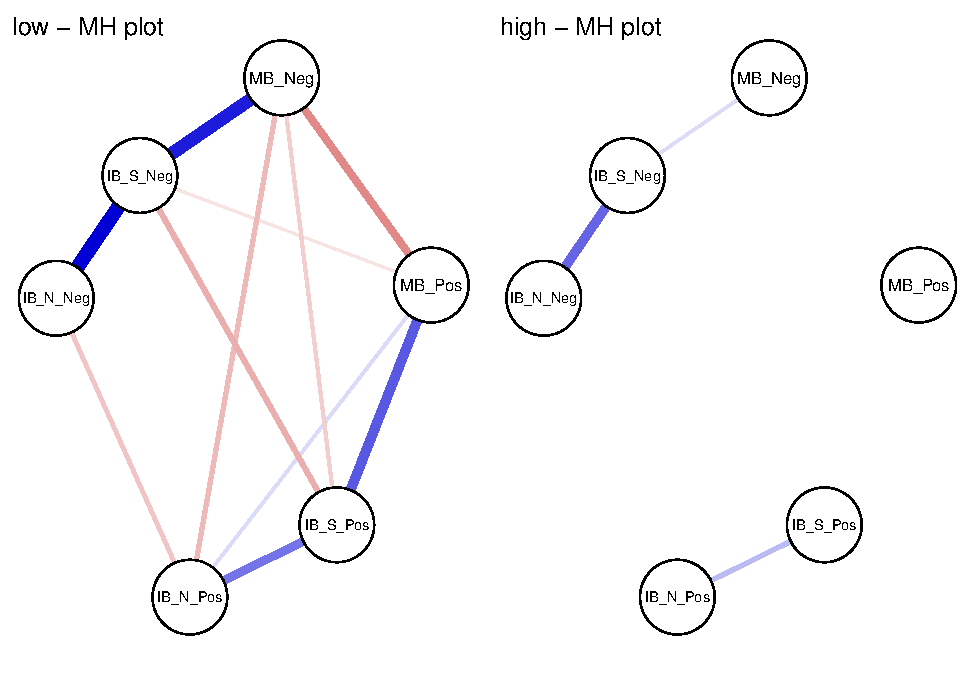
\includegraphics{supplimental_analysis_files/figure-latex/unnamed-chunk-1-1.pdf}
\caption{\label{fig:unnamed-chunk-1}Graphical LASSO Networks. The left and right panels present the graphical LASSO network from the low mental health group and the high mental health group, respectively. Each node represents a cognitive bias measure and each edge represents the (partial) correlation between the nodes it connects, after controlling for all other variables in the network. Thicker edges represent stronger associations. Blue edges indicate positive relationships, whereas red edges indicate negative relationships.
Note. IB\_S\_Pos = Social Positive Interpretation Bias; IB\_S\_Neg = Social Negative Interpretation Bias; IB\_N\_Pos = Non-Social Negative Interpretation Bias; IB\_N\_Neg = Non-Social; MB\_Pos = positive memory bias; MB\_Neg = negative memory bias.}
\end{figure}

\newpage

\hypertarget{references}{%
\section{References}\label{references}}

\begingroup
\setlength{\parindent}{-0.5in}
\setlength{\leftskip}{0.5in}

\hypertarget{refs}{}
\leavevmode\hypertarget{ref-R-bootnet}{}%
Epskamp, S., Borsboom, D., \& Fried, E. I. (2017). Estimating psychological networks and their accuracy: A tutorial paper. \emph{Behavior Research Methods}. Retrieved from \url{https://arxiv.org/abs/1604.08462}

\leavevmode\hypertarget{ref-foygel_extended_2010}{}%
Foygel, R., \& Drton, M. (2010). Extended Bayesian Information Criteria for Gaussian Graphical Models, 1--14. Retrieved from \url{http://arxiv.org/abs/1011.6640}

\leavevmode\hypertarget{ref-friedman_sparse_2008}{}%
Friedman, J., Hastie, T., \& Tibshirani, R. (2008). Sparse inverse covariance estimation with the graphical lasso. \emph{Biostatistics}, \emph{9}(3), 432--441. \url{https://doi.org/10.1093/biostatistics/kxm045}

\leavevmode\hypertarget{ref-R-glasso}{}%
Friedman, J., Hastie, T., \& Tibshirani, R. (2019). \emph{Glasso: Graphical lasso: Estimation of gaussian graphical models}. Retrieved from \url{https://CRAN.R-project.org/package=glasso}

\leavevmode\hypertarget{ref-R-NetworkComparisonTest}{}%
van Borkulo, C. D., Sacha Epskamp, \& Millner, A. (2016). \emph{NetworkComparisonTest: Statistical comparison of two networks based on three invariance measures}. Retrieved from \url{https://CRAN.R-project.org/package=NetworkComparisonTest}

\endgroup

\end{document}
